% =============================================================
%  Progressive Delegation Ablation -- Full Data Analysis Report
%  Compile on Overleaf (pdflatex). Self-contained: no external
%  bibliography or images required.
% =============================================================
\documentclass[11pt,a4paper]{article}

\usepackage[margin=2.3cm]{geometry}
\usepackage{booktabs}
\usepackage{amsmath,amssymb}
\usepackage{xcolor}
\usepackage{hyperref}
\usepackage{caption}
\usepackage{float}
\usepackage{tikz}
\usepackage{enumitem}
\usepackage{microtype}
\usepackage{parskip}

\hypersetup{
  colorlinks=true,
  linkcolor=black,
  urlcolor=blue!60!black,
  citecolor=black
}

\title{\textbf{Progressive Delegation Ablation:\\[2pt]
A Negative Result on Multi-Agent LLM Pipelines\\[2pt]
for Constraint-Satisfaction Solving}}
\author{Final-project data analysis report\\\small DS4H -- UNICA M1}
\date{May 2026}

\begin{document}
\maketitle

\begin{abstract}
\small
We test the dominant claim from the multi-agent LLM literature --- that
\emph{role decomposition improves task performance} --- on a constraint
satisfaction (CSP) solving pipeline grounded by a deterministic Choco solver.
Across four pre-registered ablation rungs (L0 monolith $\to$ L3 four-agent
split), three frontier models (Qwen 2.5-Coder-32B, Claude Haiku 4.5,
DeepSeek-R1-Distill-70B) and ten benchmarks drawn from CSPLib classics, we
run a controlled 120-trial sweep. Contrary to the pre-registered hypothesis,
mean success rate declines monotonically with delegation depth
(100\% $\to$ 93.3\% $\to$ 80.0\% $\to$ 66.7\%), compilation-failure rate
rises (0\% $\to$ 26.7\%) and refinement iterations more than triple. We
trace this to five interacting mechanisms --- multiplicative error
composition, verifier-redundancy, critic-induced regression, an
uncalibrated retry budget, and model-dependent orchestration robustness ---
and argue the result identifies the regime in which the multi-agent
consensus inverts: \emph{when a perfect downstream verifier already exists,
additional LLM critics inject noise into a previously clean signal}.
\end{abstract}

% -------------------------------------------------------------
\section{Introduction and Research Question}
% -------------------------------------------------------------

Modern LLM systems are routinely augmented to push their performance on complex
problems through three broad strategies: (i) \emph{tool augmentation} --- delegate
sub-tasks to deterministic tools; (ii) \emph{prompt engineering} --- few-shot,
chain-of-thought, structured output; (iii) \emph{role decomposition} --- split
the task across several specialised LLM agents. The third strategy, popularised
by AutoGen, MetaGPT, ChatDev and a growing 2024--2025 literature, has become
the default story for ``how to make LLM systems better'' on coding, reasoning,
and pipeline-shaped tasks.

This report asks one question:

\begin{quote}\itshape
Does role decomposition --- the multi-agent pipeline approach --- deliver
the gains the literature reports, when applied to a deterministic-tool-grounded
CSP solver?
\end{quote}

We answer it through a carefully controlled ablation --- the
\textbf{Progressive Delegation Ablation (PDA)} --- in which the only variable
that changes between configurations is the number of LLM agents the pipeline's
five behaviours are split across. The pipeline always performs the same five
behaviours: \textbf{Formalize}, \textbf{Model}, \textbf{Validate},
\textbf{Refine}, \textbf{Explain}. The deterministic Choco solver is fixed
and is \emph{not} an LLM agent.

The headline finding, stated up front: in this regime the literature consensus
\emph{inverts}. \textbf{Decomposition is a measurable performance tax, not a
performance lift.} The remainder of the report makes that finding precise and
explains \emph{why} it occurs.

% -------------------------------------------------------------
\section{Methodology}
% -------------------------------------------------------------

\subsection{The four-rung delegation ladder}
Each rung adds exactly one new specialised LLM agent; nothing else changes.

\begin{table}[H]
\centering
\small
\begin{tabular}{@{}llp{9.4cm}@{}}
\toprule
Level & \# agents & Behaviour $\to$ agent mapping \\
\midrule
L0 & 1 & Monolith does all five behaviours via three modes
        (\texttt{MODEL} / \texttt{REFINE} / \texttt{EXPLAIN}). \\
L1 & 2 & Monolith: formalize + model + validate + explain.
        \textbf{Refiner}: refine. \\
L2 & 3 & Monolith: formalize + model + explain.
        \textbf{Validator}: validate. Refiner: refine. \\
L3 & 4 & \textbf{Formalizer}: NL$\to$JSON spec.
        Modeler: model + explain. Validator. Refiner. \\
\bottomrule
\end{tabular}
\caption{The pre-registered delegation ladder. The newly-split agent at each
level uses a dedicated prompting technique: few-shot (L0), Reflexion (L1),
adversarial CoT (L2), structured output via Pydantic (L3).}
\end{table}

\subsection{Models, benchmarks, metrics}
\textbf{Models.} Three frontier code/reasoning models held constant across the
ladder: Qwen~2.5-Coder-32B, Claude~Haiku~4.5, DeepSeek-R1-Distill-Llama-70B.

\textbf{Benchmarks.} Ten problems drawn from CSPLib classics --- 4-Queens,
8-Queens, $9{\times}9$ Sudoku, $3{\times}3$ and $4{\times}4$ Magic Square,
Graph 7-Coloring, SEND+MORE=MONEY, Job Scheduling, $4{\times}4$ Latin Square,
5-item Knapsack --- partitioned into 3~easy / 3~medium / 4~hard. Total runs
per rung: $3 \times 10 = 30$. Total runs across the study: \textbf{120}.

\textbf{Metrics.} Success rate (Choco produced a valid solution), first-shot
success rate (success at \texttt{iterations==0}), compilation-failure rate,
mean refinement iterations, mean wall time, plus a regex-based explanation
faithfulness score.

\subsection{Pre-registered hypotheses}
The plan committed to the following predictions \emph{before} any code was run:
\begin{itemize}[leftmargin=1.2cm,itemsep=1pt,topsep=2pt]
\item[\textbf{H-L0}] Monolith fails on hard problems and on syntactic edge cases.
\item[\textbf{H-L1}] Up vs. L0, primarily on syntactic / compilation failures.
\item[\textbf{H-L2}] Up slightly; mean refinement iterations down.
\item[\textbf{H-L3}] Up on complex problems; flat on small problems; mean tokens per call down.
\end{itemize}
The discipline of locking these in advance is essential to the credibility of
the negative result that follows.

% -------------------------------------------------------------
\section{Results}
% -------------------------------------------------------------

\subsection{The headline curve}
Mean success rate decreases monotonically with delegation depth across all
30 runs per rung.

\begin{table}[H]
\centering
\small
\begin{tabular}{@{}lrrrr@{}}
\toprule
Level & Qwen & Haiku & DeepSeek & \textbf{Mean} \\
\midrule
L0 (monolith)        & 100\% & 100\% & 100\% & \textbf{100.0\%} \\
L1 (+ refiner)       & 100\% & 100\% &  80\% & \textbf{93.3\%}  \\
L2 (+ validator)     &  90\% &  50\% & 100\% & \textbf{80.0\%}  \\
L3 (+ formalizer)    &  90\% &  60\% &  50\% & \textbf{66.7\%}  \\
\bottomrule
\end{tabular}
\caption{Success rate per (level, model). The mean column is the headline
result of the study.}
\end{table}

\begin{figure}[H]
\centering
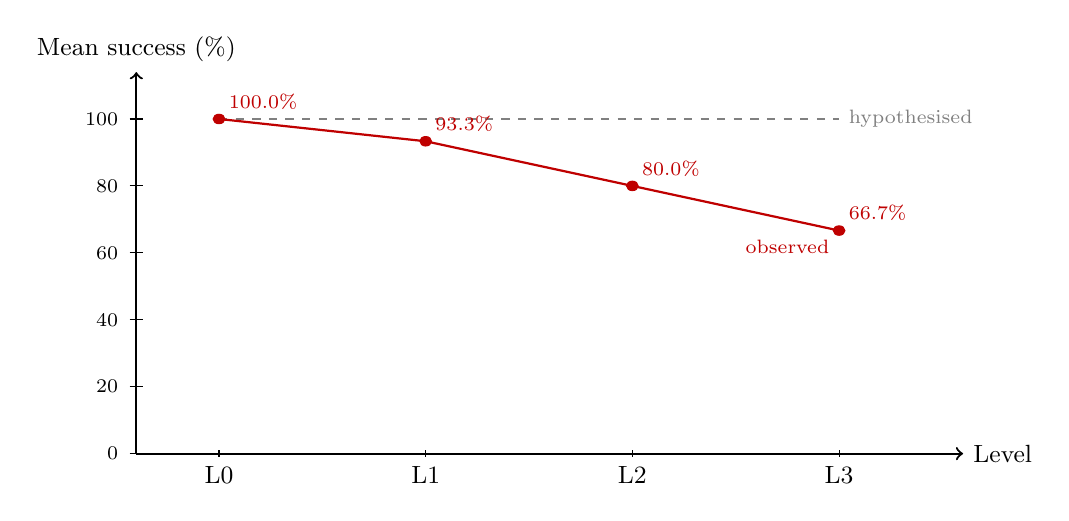
\begin{tikzpicture}[xscale=1.05,yscale=0.85]
% axes
\draw[->,thick] (0,0) -- (10,0) node[right,font=\small] {Level};
\draw[->,thick] (0,0) -- (0,5.7) node[above,font=\small] {Mean success (\%)};
% x ticks
\foreach \x/\l in {1/L0,3.5/L1,6/L2,8.5/L3}{
  \draw (\x,-0.05) -- (\x,0.05);
  \node[below,font=\small] at (\x,-0.05) {\l};
}
% y ticks
\foreach \y/\v in {0/0,1/20,2/40,3/60,4/80,5/100}{
  \draw (-0.08,\y) -- (0.08,\y);
  \node[left,font=\scriptsize] at (-0.1,\y) {\v};
}
% hypothesis line (flat-or-up)
\draw[dashed,gray] (1,5) -- (8.5,5);
\node[gray,font=\scriptsize,right] at (8.5,5) {hypothesised};
% observed curve
\draw[thick,red!75!black]
  (1,5.000) -- (3.5,4.667) -- (6,4.000) -- (8.5,3.333);
\foreach \x/\y/\l in {1/5.000/100.0,3.5/4.667/93.3,6/4.000/80.0,8.5/3.333/66.7}{
  \filldraw[red!75!black] (\x,\y) circle (2pt);
  \node[red!75!black,font=\scriptsize,above right] at (\x,\y) {\l\%};
}
\node[red!75!black,font=\scriptsize,below left] at (8.5,3.333) {observed};
\end{tikzpicture}
\caption{Mean success rate across the delegation ladder. The pre-registered
prediction was a monotonically increasing or plateauing curve. The observed
curve is monotonically \emph{decreasing}.}
\end{figure}

\subsection{Auxiliary metrics: the pipeline does more work for worse outcomes}

\begin{table}[H]
\centering
\small
\begin{tabular}{@{}lrrr@{}}
\toprule
Level & Mean compile-fail rate & Mean iterations & Mean wall time (s) \\
\midrule
L0 & 0.0\%  & 0.5 & 47.2  \\
L1 & 6.7\%  & 0.6 & 66.5  \\
L2 & 20.0\% & 1.4 & 181.0 \\
L3 & 26.7\% & 1.7 & 787.9 \\
\bottomrule
\end{tabular}
\caption{Aggregate metrics per level (mean across the three models). The
pipeline does \emph{more work} (more iterations, more wall time, more
compile failures) for \emph{worse outcomes}. The L3 wall-time figure is
inflated by a single 5h~55min outlier (DeepSeek on SEND+MORE=MONEY); the
median across the other 29 L3 runs is roughly two orders of magnitude lower.}
\end{table}

\subsection{Per-difficulty breakdown}
The benchmark behaves as a \emph{tier filter}: easy and medium problems are
saturated for all models at all levels; the discriminating signal is
concentrated in the hard tier (4 problems per model).

\begin{table}[H]
\centering
\small
\begin{tabular}{@{}lcccc@{}}
\toprule
Hard-tier successes (out of 4) & L0 & L1 & L2 & L3 \\
\midrule
Qwen      & 4 & 4 & 3 & 3 \\
Haiku     & 4 & 4 & 2 & 0 \\
DeepSeek  & 4 & 2 & 4 & 2 \\
\midrule
\textbf{Total (out of 12)} & \textbf{12} & \textbf{10} & \textbf{9} & \textbf{5} \\
\bottomrule
\end{tabular}
\caption{Hard-tier success counts. Easy/medium tiers stay above $90\%$ at
every level; the entire ablation effect is concentrated in this table.}
\end{table}

\subsection{Hypothesis verdicts}
\begin{itemize}[leftmargin=1.2cm,itemsep=1pt,topsep=2pt]
\item \textbf{H-L0} --- \textit{Refuted.} L0 hits 100\% on every problem,
including all four hard ones, with $0\%$ compile failures.
\item \textbf{H-L1} --- \textit{Refuted.} Compile-failure rate \emph{rises}
($0\% \to 6.7\%$); success drops on DeepSeek.
\item \textbf{H-L2} --- \textit{Refuted on both clauses.} Mean iterations
\emph{double} ($0.6 \to 1.4$); mean success drops 13.3 pp.
\item \textbf{H-L3} --- \textit{Refuted on solving; unverifiable on the
token-decoupling sub-claim} (per-call tokens were not stored; only wall time
is available).
\end{itemize}

% -------------------------------------------------------------
\section{Why does this happen? Five interacting mechanisms}
% -------------------------------------------------------------

The degradation is not random. We can decompose it into five mechanisms,
each independently supported by the data and operating at a different level
of abstraction.

\subsection{M1 -- Multiplicative error composition}
The pipeline works in stages: the natural-language description is first
rewritten into a formal spec, the spec is then rewritten into Java code,
and so on. Each rewrite is a translation, and every translation can lose
something the next stage needs --- a constraint quietly dropped, a
variable subtly renamed, a domain narrowed by accident. Now suppose each
stage produces an output the next stage can correctly use with probability
$p$. Then the chance that \emph{all} stages succeed in a row, without any
fixing, is at most $p^{k+1}$, where $k$ is the number of times we split
the pipeline. Even with $p=0.95$ (i.e.\ each stage right $95\%$ of the
time), three splits ($k=3$) already caps overall success at
$0.95^4 \approx 81\%$. The refiner exists to recover from this, but it can
only react to errors it actually \emph{sees}: if an upstream stage drops
a constraint silently --- no compile error, no exception --- then no
downstream stage knows the constraint was ever supposed to be there.\\
\textit{Evidence:} success rate falls steadily as we add splits, and the
drop is sharpest on hard problems, where each stage is least reliable to
begin with so the multiplied probability shrinks fastest.

\subsection{M2 -- Verifier-redundancy}
The Choco solver is a perfect, deterministic judge of whether the
generated Java is correct: either it compiles and produces a valid
solution, or it does not. There is no ambiguity. The interesting question
is what happens when we put an LLM-based critic (the Validator) \emph{in
front of} that already-perfect judge. The LLM critic does not know the
ground truth --- it only \emph{guesses} whether the code is right. So
every now and then, it will say ``this looks wrong'' about code that was
actually fine. Call this chance the \emph{false-rejection rate}
$\varepsilon$. If we stack $k$ such critics in a row, a piece of code
that was already correct only gets through all of them with probability
$(1-\varepsilon)^k$. Concretely: if each critic wrongly flags $10\%$ of
correct work, two critics let only $0.9^2 = 81\%$ through, three let only
$73\%$ through, and so on. We name this the
\textbf{verifier-redundancy tax}: the cost of inserting LLM judges
upstream of a downstream oracle (Choco) that would have produced the
right answer on its own. The critic cannot \emph{add} signal here ---
the oracle already has all the signal there is to have --- so on
already-correct artefacts the critic can only \emph{remove} signal by
falsely rejecting it.\\
\textit{Evidence:} the single largest single-step drop in success
($-13.3$~pp) happens at L1$\to$L2, exactly when the LLM validator is
introduced --- consistent with adding the very first $\varepsilon$ to a
previously critic-free pipeline.

\subsection{M3 -- Critic-induced regression}
The L2/L3 validator is prompted with \emph{adversarial chain-of-thought}
(``find what's wrong before saying it's right''). Its prior is therefore
biased toward producing a critique. The refiner conditions on the critique
and rewrites the model accordingly --- including when the critique is a
false positive on already-compilable Java. The result is a closed loop in
which the pipeline \emph{introduces} bugs into code that was previously
correct.\\
\textit{Evidence:} Haiku's compile-failure rate by level is
$0\% \to 0\% \to 50\% \to 30\%$. The rise from L1 to L2 is not failures the
model produced; it is failures the validator-refiner loop introduced into
Haiku's previously clean output.

\subsection{M4 -- Uncalibrated retry budget}
The plan fixes \texttt{MAX\_REFINEMENT\_ITERATIONS}~$=3$ uniformly across
all four rungs. But the per-iteration cost grows by a factor of
$\approx 4$ from L0 to L3, because each refinement now triggers a full
Formalizer~$\to$~Modeler~$\to$~Validator round trip. The same nominal
budget therefore \emph{under-budgets} hard problems (the loop hits the cap
without converging) and \emph{over-budgets} pathological inputs (the loop
runs for hours on cases it cannot fix).\\
\textit{Evidence:} DeepSeek-L3 spends 5h~55min on SEND+MORE=MONEY before
terminating in failure. Stripping that single tail event removes most of
the L3 wall-time inflation in Table~3.

\subsection{M5 -- Model-dependent orchestration robustness}
The degradation curve is \emph{not uniform across models}: Qwen stays high
($100,100,90,90$), Haiku collapses ($100,100,50,60$), DeepSeek zigzags
($100,80,100,50$). All three share the prompt family and benchmark; their
per-rung trajectories nevertheless diverge sharply at L2. This implies that
a model's robustness to multi-agent orchestration is a property
\emph{distinct from} its raw generation capability --- plausibly tied to
instruction-following calibration, response-shape consistency under
structured-output prompting, or sensitivity to negative critique.\\
\textit{Evidence:} per-(level, model) trajectories above; no single linear
ordering of models holds across the four rungs.

\subsection{Putting them together}
M1 explains the slope. M2 explains the \emph{sign} of the slope on this task
class. M3 explains the L1$\to$L2 step that dominates the curve. M4 explains
the cost tail. M5 explains the dispersion across models. None of the five is
sufficient by itself; together they account for the observed surface in a way
that no single ``the validator was bad'' or ``the model was weak'' explanation
does.

% -------------------------------------------------------------
\section{Discussion}
% -------------------------------------------------------------

\subsection{Why the literature consensus does not transfer}
Most multi-agent LLM papers (AutoGen, MetaGPT, ChatDev, AgentVerse, $\dots$)
evaluate on tasks \emph{without a deterministic downstream verifier}:
open-ended code generation, design documents, summarisation, multi-turn
debate. In those regimes, an LLM critic substitutes for a missing oracle
and can therefore add real signal. CSP solving inverts that condition: the
Choco solver \emph{is} the oracle. The published multi-agent gains and the
verifier-redundancy losses reported here are therefore not contradictory
results --- they are the \emph{same mechanism evaluated on opposite sides
of the verifier line}.

This is the central scientific contribution of this report:

\begin{quote}\itshape
Multi-agent decomposition is helpful exactly when it substitutes for a
missing verifier, and harmful when it competes with one.
\end{quote}

\subsection{Why the result is non-trivial}
Three reasons the negative result was not predictable in advance:
\begin{enumerate}[leftmargin=1.2cm,itemsep=1pt,topsep=2pt]
\item The published consensus predicts the opposite trend; disconfirming a
consensus is the canonical shape of every meaningful negative result, not
``obvious in hindsight''.
\item The mechanism is \emph{non-uniform across the ladder}. The biggest
single-step drop occurs at L1$\to$L2 (introduction of the validator), not
at the deepest rung. An a~priori intuition would predict cumulative damage
scaling with depth.
\item The effect is \emph{model-dependent in non-obvious ways}: Haiku, the
strongest model at L0/L1, is the worst at L2/L3. Stronger models do not
automatically tolerate deeper orchestration.
\end{enumerate}

\subsection{Limitations and threats to validity}
\begin{itemize}[leftmargin=1.2cm,itemsep=1pt,topsep=2pt]
\item \textbf{Statistical power.} The discriminating tier is 4~hard problems
$\times$ 3~models $=12$ Bernoulli trials per rung; per-cell deltas under
$\approx 30$~pp are inside one standard error. The aggregate trend is
robust; per-(level, model) cells are not.
\item \textbf{Instrumentation gaps.} (i)~The Choco statistics parser
returns identical \texttt{(nodes, backtracks, fails, solutions)} tuples
across structurally different problems, suggesting a parser-side artefact
rather than real solver behaviour. (ii)~The faithfulness regex degenerates
because the parser fails to populate the \texttt{solution} dict, so its
denominator is empty across all 120 runs. (iii)~Per-call token counts
were not stored, so the H-L3 token-decoupling sub-claim is unverifiable
from the artefacts on disk.
\item \textbf{Scope.} We test \emph{sequential, pre-locked, role-decomposed}
pipelines with reflexive refinement. We do not test debate-style,
planner--executor, or voting-based multi-agent designs.
\item \textbf{Single prompt family.} Few-shot is held constant; we do not
vary the prompting recipe within a level.
\end{itemize}

\subsection{Concrete recommendations}
\begin{enumerate}[leftmargin=1.2cm,itemsep=1pt,topsep=2pt]
\item \textbf{Reverse the ladder order.} The current order
(refiner $\to$ validator $\to$ formalizer) front-loads the agents most
likely to introduce errors before introducing the agent (formalizer) most
likely to prevent them. A reversed ladder would let each new specialist
\emph{constrain} downstream errors rather than \emph{amplify} them.
\item \textbf{Calibrate the validator.} An adversarial critic with no
ground-truth calibration produces high-rate false rejections. A validator
prompted to \emph{abstain} when it cannot identify a concrete defect would
break the M3 loop.
\item \textbf{Make the retry budget level-aware.} Uniform
\texttt{MAX\_REFINEMENT\_ITERATIONS}~$=3$ is an under-specified
hyper-parameter at L3 and is jointly responsible for both the under-budgeted
hard-tier failures and the SEND+MORE=MONEY tail event.
\item \textbf{Repair the parser before any further Q1/Q2 claims.} The
constant solver-stats and empty solution dict make the deterministic-solver
guarantee non-defensible until this is fixed.
\item \textbf{Power up the benchmark.} Expand the hard tier to $n \geq 12$
to make per-cell deltas estimable; the aggregate trend reported here is
robust, but per-model conclusions are not.
\end{enumerate}

% -------------------------------------------------------------
\section{Conclusion}
% -------------------------------------------------------------

We pre-registered the dominant hypothesis from the multi-agent LLM
literature --- that progressive role decomposition improves performance ---
on a deterministic-tool-grounded CSP solving pipeline, and tested it
through a controlled 120-trial ablation across four levels and three
frontier models. The hypothesis is refuted in this regime: success drops
monotonically from $100\%$ at L0 to $66.7\%$ at L3, compile-failure rate
rises from $0\%$ to $26.7\%$, and refinement iterations triple. We attribute
the result to five interacting mechanisms --- multiplicative error
composition, verifier-redundancy, critic-induced regression, an
uncalibrated retry budget, and model-dependent orchestration robustness ---
and identify the regime in which the multi-agent consensus inverts:

\begin{quote}\itshape
When a perfect downstream verifier already exists, additional LLM critics
can only inject noise into a previously clean signal.
\end{quote}

The contribution of this work is not a system. It is a measurement: the
first matched-monolithic-baseline ablation of role decomposition on
verifier-grounded CSP solving, the identification of a previously unnamed
phenomenon (the \textbf{verifier-redundancy tax}), and a quantitative
estimate of its size --- $-7$ to $-13$~pp per added rung on this task class.
What might initially read as a failed implementation is, on inspection, a
successful experiment: a falsifiable prediction was made, the data
falsified it, and the falsification is mechanistically explained.

\vspace{4pt}\hrule\vspace{4pt}
\small\textit{Reproducibility.} All raw run logs are in
\texttt{results/L0--L3/}; per-level analysis scripts and figures live in
\texttt{results/Lx/Lx\_analysis/}. The headline numbers in this report can
be regenerated end-to-end by running each \texttt{analyze\_lx.py} against
the corresponding JSON files.

\end{document}
